\section{Efficient Parallel Heap Implementation}
\label{s:impl}

Like an array representation, a heap can be represented by hardware registers or FPGA latches.
An array of latches can virtually represent each level of a heap.
The number of latches at each level can be represented as $2^{\beta_k-1}$, where $\beta_k$ is the $k^{th}$ level, assuming that root is in level $1$.
Figure \ref{fig5} shows how latches represent levels.
In this example, the root node is stored in $L_1$; two elements are stored in the next level, $L_2$; the level after that is $L_3$, storing four elements; and the last level, $L_4$, has three elements, although it can have a maximum of eight.

\begin{figure}[!ht]
  \centering
  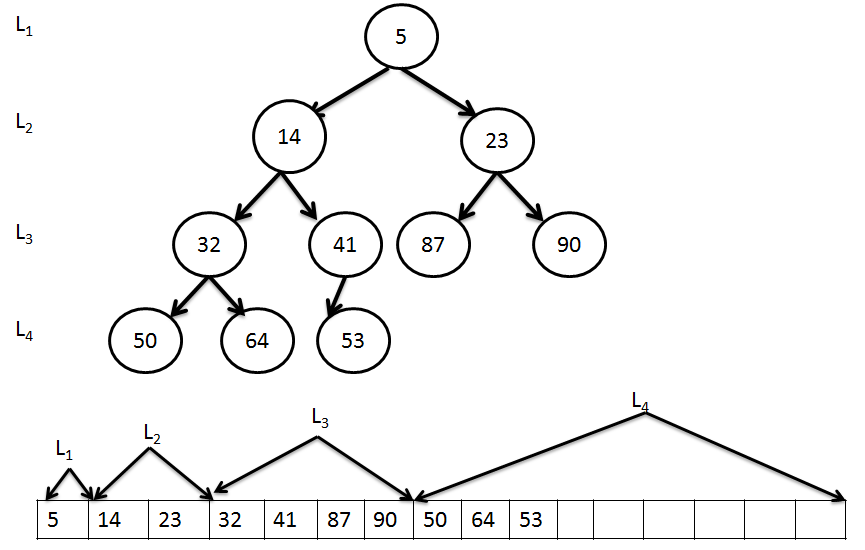
\includegraphics[width=6cm]{fig/5.png}
      \caption{Storage in FPGA of different nodes in binary heap}
    \label{fig5}
\end{figure}

\begin{figure}[!ht]
  \centering
  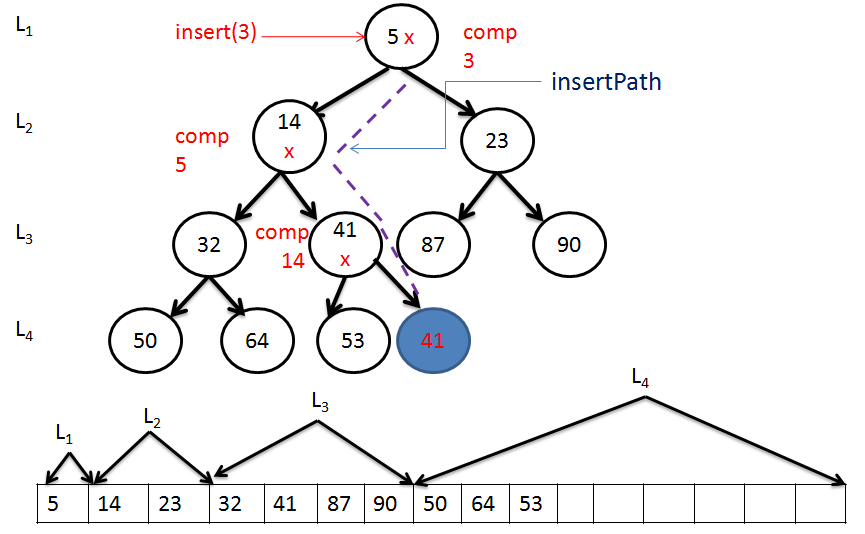
\includegraphics[width=6.5cm]{fig/6.png}
      \caption{Insert path}
    \label{fig6}
\end{figure}

\begin{figure}[!ht]
  \centering
  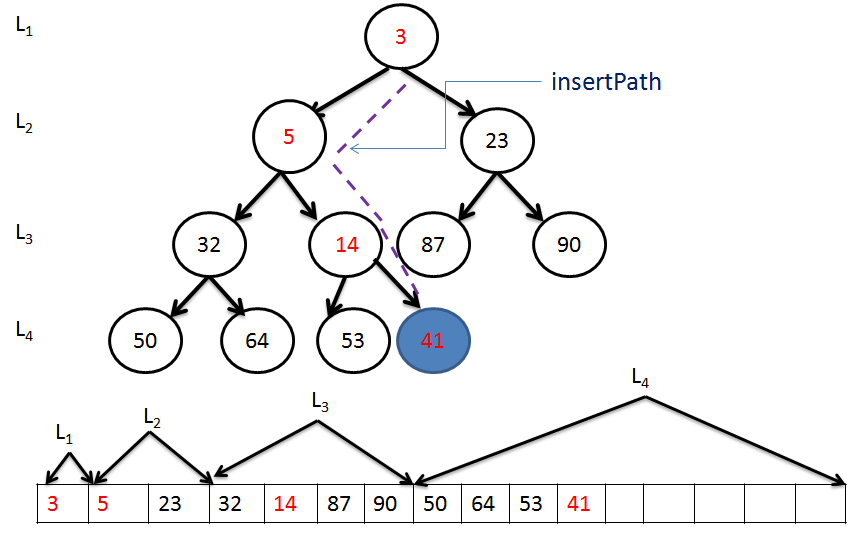
\includegraphics[width=6.5cm]{fig/7.png}
      \caption{Container of latches $L$ after insertion completes.}
    \label{fig7}
\end{figure}

\subsection{Insert Operation}

The {\it insert} operation, which is intimated from the last available node of a heap.
However, if a bottom-up insertion is done in parallel with other operations such as {\it min-delete}, it may cause an inconsistency in the heap.
To clarify, let us consider the example in Figure \ref{fig5}.
Suppose we insert element $3$ into the heap and then immediately delete one element.
Let us assume nodes at each level get updated in a single clock cycle.
That means, in the worst case, a total of four clock cycles is required to complete only an insert operation in this situation.
Before it completes, if a {\it min-delete} comes, that operation has to wait up to four clock cycles to avoid deleting a wrong element from the root (5 in this case).
Thus, it is incumbent to insert from the root and go down.
However, we need to know the exact path for the newly inserted element, otherwise the tree will no longer hold the conditions of a complete binary tree.
We adopt an algorithm presented by Vipin {\it et. al} \cite{pq6} in our design. The algorithm is as follows:

\begin{enumerate}
\item Let $k$ be the last available node where a new element can be placed. Let $j$ be the first node of the last level. Then, the binary representation of $k-j$ will give the path for the insertion.
\item Let $k-j = B$, and represent $B$ in binary form $b_{\beta-1}b_{\beta-2} \cdots b_2b_1$. Starting from root, scan each bit of $B$ starting from $b_{\beta-1}$;
    \begin{itemize}
    \item {\bf if} $b_i == 0$ ($i \in \{\beta-1,\beta-2, \cdots, 2,1$), {\bf then} go to left
    \item {\bf else} go right
    \end{itemize}
\end{enumerate}

Figure \ref{fig6} shows the insert path for a new element $3$. In this case, the node at index $11$ should be filled up.
The first node of the last level is at index $8$.
So, $11 - 8 = 3$, which can be represented as 011 in binary.
Starting from root, the path should be $root \rightarrow left \rightarrow right \rightarrow right$, as illustrated by the Figure \ref{fig6}. Figure \ref{fig7} represents the binary tree and latches after this insert operation.

\subsection{Min-Delete Operation}

There is one conventional approach to delete an element from a heap.
Since a min element resides at the root, deletion always happens from the root, and the last element of the heap replaces the root.
There are two difficulties here:

\begin{enumerate}
\item For sequential operation, this method works fine. Parallel execution of insert/delete, however, can create a hole. This happens after any {\t insert} followed by {\it min-delete}.
\item Replacing the root with the last element of the heap requires an additional clock cycle to write that element into the root node. Additionally, we need to compare three elements: root and its two children, or any node and its children. From a hardware perspective, it is cost-efficient to compare two elements rather than three. Moreover, 3-element comparisons cause a longer path delay.
\end{enumerate}


\begin{figure}[!ht]
  \centering
  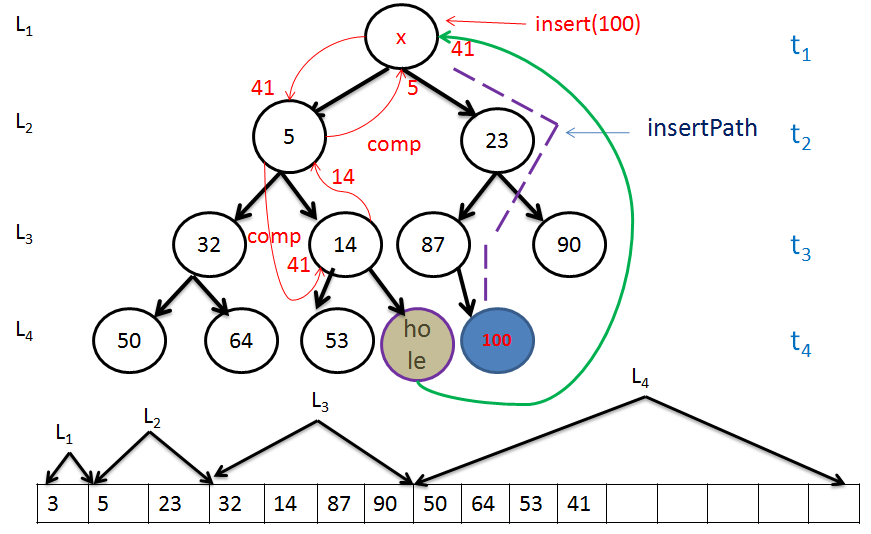
\includegraphics[width=6.5cm]{fig/8.png}
      \caption{A hole results from parallel operation of insert-delete}
    \label{fig8}
\end{figure}

\begin{figure}[!ht]
  \centering
  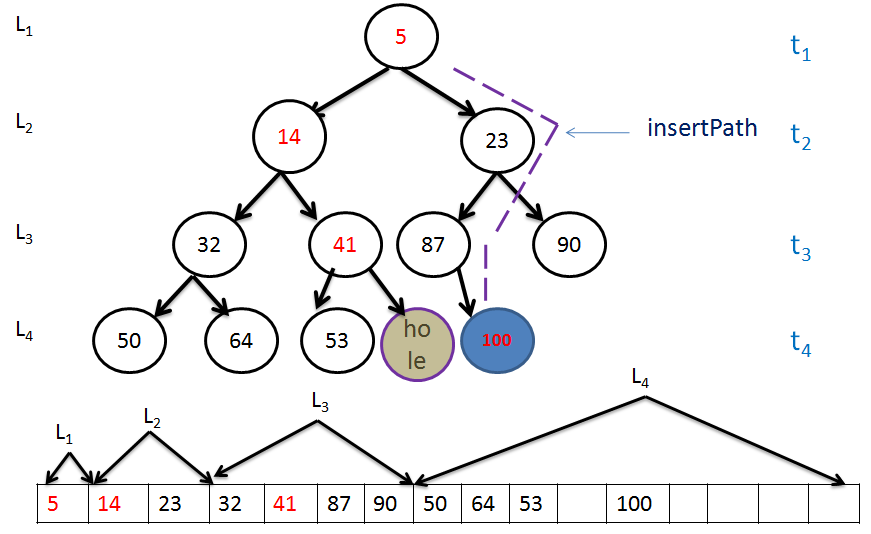
\includegraphics[width=6.5cm]{fig/9.png}
      \caption{Container of latches ($L$) after parallel operation of insert-delete}
    \label{fig9}
\end{figure}

\begin{figure*}[!ht]
  \centering
  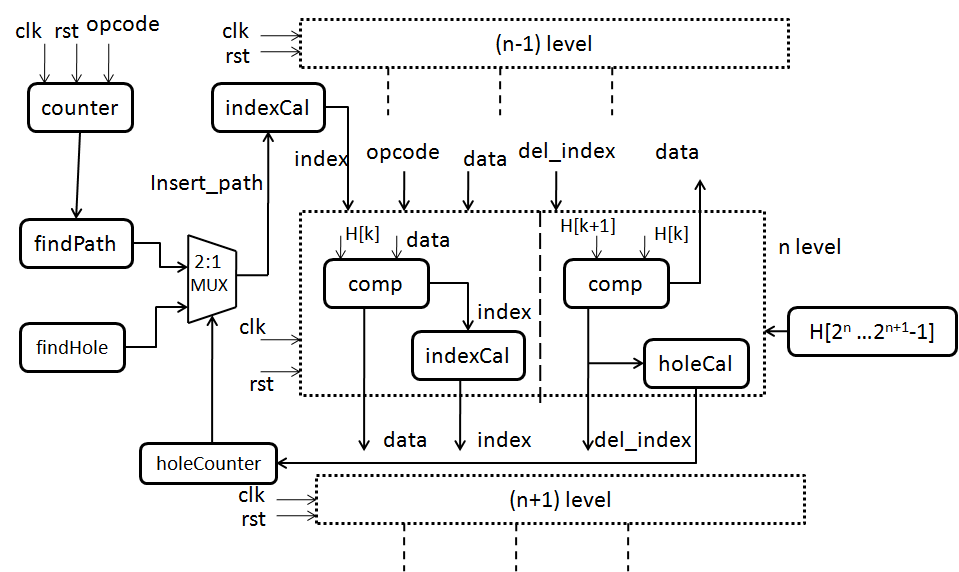
\includegraphics[width=9.5cm]{fig/2.png}
      \caption{Top Level Architecture of insert-delete}
    \label{fig10}
\end{figure*}

Figure \ref{fig8} illustrates the first issue clearly.
Here, an insert-delete combination is performed on the heap from Figure \ref{fig7}.
At time $t_1$, the insert operation with element $100$, denoted by $insert(100)$, is encountered.
The element will be inserted at the last node of the last level, which is at index $12$.
After one clock cycle of {\it insert}, {\it min-delete} is encountered at $t_2$.
But, at that time, $insert(100)$ is being processed at level $L_2$, so the last element is still the $11^{th}$ node.
The min-delete operation will create a hole at the $11^{th}$ node, as shown in Figure \ref{fig8}.
Eventually, when $insert(100)$ finishes, element $100$ will occupy at the position of $H[12]$, but $H[11]$ will become empty.
Figure \ref{fig9} illustrates this situation.

Let us assume that an insert operation comes at time $t_i$ and a min-delete operation comes at $t_j$, where $i, j = 1,2,3, \cdots$ and $j>i$.
All operations take one clock cycle at any level to complete their respective tasks at that level.
Only a single node, if any, gets modified for all levels.
In general, any insert-delete combination will create a hole if $(t_j - t_i) < \beta\tau$, where $\beta$ is the depth of the heap and $\tau$ is the cycle time per level.

The naive approach to avoid a hole from an insert-delete combination is to stall {\it min-delete} from entering the pipeline until {\it insert} completes.
After insertion completes, the last element will update to the newly filled node.
Thus, when the delete operation begins, the heap will correctly identify the new node as the last element to replace the root with instead of the node before.
However, this method turns every {\it insert} that is followed by a {\it min-delete} into a sequential operation.
The number of cycles the delete operation must wait for the insert operation to complete depends on the heap's depth.
In the worst-case scenario, where a binary heap of many levels encounters a sequence containing only insert-delete combinations, performance degrades significantly.

To solve the first issue, we propose a hole minimization technique.
With this technique, the holes are removed while an insert operation is processed.
We check for the existence of a hole by checking a special-purpose register, and if one exists, we fill it with the new element.
We apply the insert algorithm, except we modify it so that the data will be inserted at the position of a hole instead of the last available node.
In the case of multiple holes, we fill the last hole with inserted data for implementation ease.
Details of this algorithm are described in the next subsection.

To address the second issue, we intentionally avoid the root replacement by the last element.
We delete root first and keep it as it is.
Then, we fill the root with its least child and follow the min-delete algorithm described in the previous section.
This way, we can save one cycle and minimize the path delay.

\subsection{Insert-Delete Logic Implementation}

{\it Insert-delete} logic is implemented to realize the proposed priority queue.
The logic handles the {\it insert} and {\it min-delete} operations for each level.

\begin{algorithm}
\label{algo1}
        \caption{$Insert-Delete (data, opcode)$}
\label{algo1}
        \begin{algorithmic}[1]
           % \Procedure{Insert}{data,opcode} %\Comment{The g.c.d. of a and b}
          \IF{($opcode$ $==$ INSERT)} %\rcomment{Insertion}
            \STATE{$counter$ $=$ $counter$ $+$ $1$}
            \STATE{($insert\_path$, $holeCounter$) $=$ $findPath$($counter$, $holeCounter$)}
            \FOR{($i = 1$ \TO $\beta$) }
                \STATE{$index$ $=$ $indexCal$($insert\_path$, $i$, $index$)}
                \IF{($data < H[index]$}
                    \STATE{swap $H[index]$ and $data$\\
                    }
                \ENDIF
            \ENDFOR
          \ELSE
          \STATE {
          $H[1]$ $=$ NULL \\
          }
          \WHILE{($leftChild[del\_index]$ $\neq$ NULL $\&\&$ $rightChild[del\_index]$ $\neq$ NULL)}
            \IF{(leftChild[del\_index] $<$ rightChild[del\_index])}
                \STATE{$H[del\_index]$ $=$ $leftChild[del\_index]$\\
                $del\_index = del\_index *2$
                }
            \ELSE
                \STATE{$H[del\_index]$ $=$ $rightChild[del\_index]$\\
                $del\_index$ $=$ $del\_index *2 + 1$
                }

            \ENDIF

          \ENDWHILE
          \STATE{ $counter = counter - 1$\\
          $holeCounter = holeCounter + 1$\\
          $holeReg[holeCounter] = del\_index$
          }
        \ENDIF

        \end{algorithmic}
\end{algorithm}

\begin{algorithm}
\caption{$findPath$($counter$, $holeCounter$)}
\label{algo2}
\begin{algorithmic}[1]
    \IF{($holeCounter > 0$)}
        \STATE{$holeCounter = holeCounter - 1$\\
        \RETURN ($holeCal(holeCounter)$, $holeCounter$)\\
        }
    \ELSE
        \STATE{$leaf\_node$ = $findNode(counter)$ \\
        \RETURN ($counter - leaf\_node$, $holeCounter$)
        }
    \ENDIF
\end{algorithmic}
\end{algorithm}

\begin{algorithm}
\caption{$findNode(counter)$}
\label{algo3}
\begin{algorithmic}[1]
    \FOR{($i = 1$;  $2^i \leq counter$; $i = i + 1$) }
        \STATE{$leaf\_node = i + 1$}
    \ENDFOR
    \RETURN $leaf\_node$
\end{algorithmic}
\end{algorithm}

\begin{algorithm}
\caption{$holeCal(holeCounter)$}
\label{algo4}
\begin{algorithmic}[1]
    \RETURN $holeReg[holeCounter]$
\end{algorithmic}
\end{algorithm}

\begin{algorithm}
\caption{$indexCal$($insert\_path$, $level$, $index$)}
\label{algo5}
\begin{algorithmic}[1]
    \IF{($bit_{level}$ of $insert\_path$ $==$ $0$)}
        \RETURN{$index$ $=$ 2*$index$}
    \ELSE
        \RETURN{$index$ $=$ 2*$index + 1$}
    \ENDIF
\end{algorithmic}
\end{algorithm}

Figure \ref{fig10} illustrates the top-level architecture of the priority queue employing the insert-delete logic.
The {\it counter} maintains the total number of elements present in the heap.
It is incremented by one for an insert operation and decremented by one for a min-delete operation.
Modifying the existing path-finding algorithm proposed by \cite{pq6}, we consider {\it holeReg} during insertion to obtain the insert path.
The {\it holeReg} contains holes created from min-delete operations.
We maintain {\it holeCounter} to identify a valid hole with {\it holeReg}.
The {\it indexCal} block finds the insert path.
The heap node at {\it index} is accessed and compared to the present data.
Based on the comparison, either the present data updates the node and the previous node data is passed to the next level, or the node remains unchanged and the present data is passed to the next level.


\begin{figure}[!ht]
  \centering
  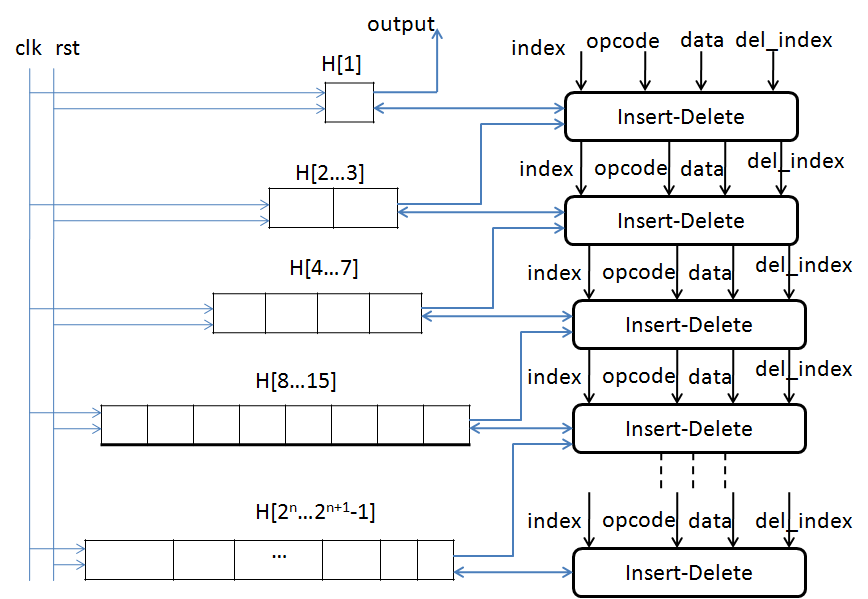
\includegraphics[width=7.5cm]{fig/1.png}
      \caption{Pipeline design overview}
    \label{fig11}
\end{figure}

%{\bf Deletion :}
We also maintain {\it del\_index} to find the last deleted node.
For example, initially, {\it del\_index} is $1$, meaning the root is deleted.
%Original version: The comparator finds the min element between $H[del\_index*2]$ and $H[del\_index*2 + 1]$, and that min element is replaced with $H[del\_index]$.
The comparator finds the min element between $H[del\_index*2]$ and $H[del\_index*2 + 1]$, and that min element replaces $H[del\_index]$.
Now, {\it del\_index} updates to the index of min element.
%Original version: Again, the comparator finds the min of the ancestors of the new index and replaces the node of the new index with that of the min element.
Again, the comparator finds the min child from the new index and replaces the node at the new index with that of the min element.
Each time, {\it holeCal} determines whether a valid child exists for {\it del\_index}.
If not, then {\it holeCounter} is incremented by 1, and {\it holeReg} is updated with {\it del\_index}.
In this manner, we maintain {\it hole}.

Algorithm \ref{algo1} presents the insert-delete parallel algorithm.
We use a 2:1 multiplexer to select the path based on the value of {\it holeCounter}.
The logic for {\it findPath} is illustrated in Algorithm \ref{algo2}.
Within {\it findPath}, the {\it findNode} logic calculates the first node of the last level.
That node can be determined using the mathematical expression $log(n)$ rounded down, where $n$ is the number of elements in the binary heap.
%There is some difficulty to realize this expression in hardware.
Algorithm \ref{algo3} presents the hardware implementation of this logic.
The {\it indexCal} block uses the output of {\it findPath} as well as the current level and index to generate the next index for the insertion path. Algorithm \ref{algo5} illustrates this logic.
Functionally, {\it holeCal} is an implementation of a stack register. Its return value is presented at Algorithm \ref{algo4}.

%We use a global clock (clk) and a global reset (rst) signal for the each logic block except the combinational logic parts. The clk and rst signals are not mentioned at each figure due to place limitation.


\subsection{Pipeline Design}
\begin{figure*}[!ht]
  \centering
  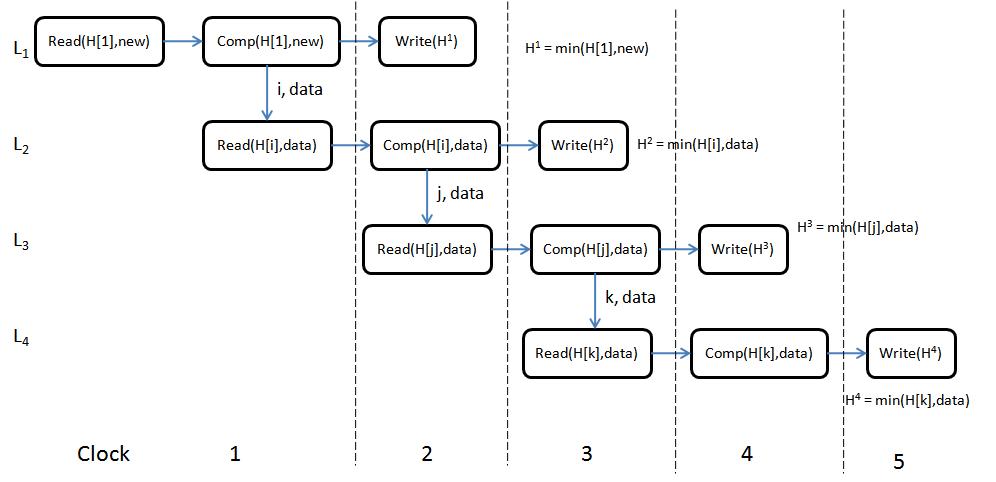
\includegraphics[width=12cm]{fig/clock1.png}
      \caption{Parallel insert operation: illustrates operations at each level at each clock }
    \label{clock1}
\end{figure*}

\begin{figure*}[!ht]
  \centering
  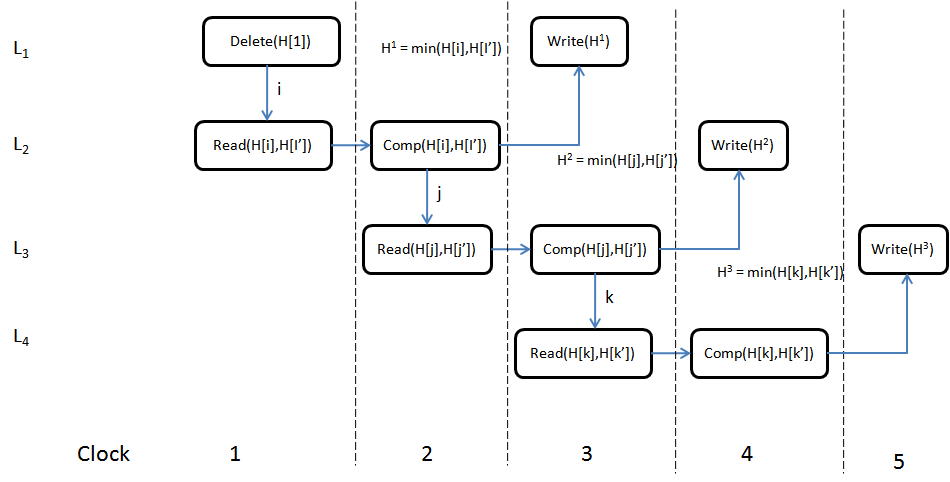
\includegraphics[width=12cm]{fig/clock2.png}
      \caption{Parallel delete operation: illustrates operations at each level at each clock.  }
    \label{clock2}
\end{figure*}

To achieve high throughput, we need to start one operation before completing the previous so that multiple operations can be in progress at the same time.
Figure \ref{fig11} illustrates the basic pipeline architecture of our binary heap.
Each level executes {\it insert} or {\it min-delete} based on signal {\it opcode}, and only one operation can be executed there at any given time $t$.
It sends {\it data} and {\it opcode} to the next level to perform.
All levels, except the first, contain the same logic hardware.

Within an operation, each level has to perform three tasks in this order: {\it read}, {\it compare}, and {\it write}.
Each task individually takes one clock cycle to execute, meaning each insert or min-delete operation performs three cycles of meaningful work at a level.
During {\it comp}, the level sends the data and opcode to the next level so that the latter can begin its tasks.
{\it Comp} for one level and {\it read} for the next level is started at positive edge and negative edge of the same clock cycle respectively. This way, the next level can read the data and opcode generated from the previous level at the next clock cycle while the previous performs {\it write}.


Figure \ref{clock1} illustrates the pipeline flow for a parallel insert operation, broken down to the three tasks.
Generally, at any level, $L_i$, if {\it read} performs at time $t$, then {\it comp} completes there at $t+1$.
The comp task generates the next {\it index} to be read by the next level, $L_{i+1}$, which performs {\it read} at $t+1$.
At $t+2$, $L_i$ performs {\it write}, and $L_{i+1}$ finishes {\it comp}, which generates the index to be read by $L_{i+2}$.
At $t+3$, $L_i$ can accept a new operation, $L_{i+1}$ performs {\it write}, and $L_{i+2}$ completes {\it comp}, which generates the index for $L_{i+3}$. 
The pattern repeats for subsequent levels until the insert operation finishes.
Effectively, this results in a {\it write} at each clock cycle after an initial latency of two clock cycles at the first level.


Figure \ref{clock2} illustrates a parallel min-delete operation. 
In all levels except the first, {\it read} and {\it write} behave similarly as with the insert operation.
However, level $L_i$ does not perform {\it write} at $t+2$ but at the following cycle, $t+3$, instead.
This is because in our min-delete algorithm, the last element of the last level does not replace root after the root data is removed, so the min child has to move up to the empty node on each level.
As the min child is determined by {\it comp} in the next level $L_{i+1}$, $L_i$ has to wait one cycle so that the comparison result from $L_{i+1}$ can be written to $L_i$.
That means $L_i$ suffers a temporary hole at $t+2$.
This hole is filled as $L_{i+1}$ writes to $L_i$ at $t+3$.
However, $L_{i+1}$ also suffers a temporary {\it hole}, but it is compensated by the next level and so on.


\subsection{Optimization Techniques}
% An {\it insert} or {\it min-delete} operation of any level waits for data from its previous level.
% As the min element of certain levels goes up to the upper level, the data will be available to write after performing a {\it comp} operation of that level.
% At all levels except root, if a {\it read} operation is executed at $t$ time by level $L_i$, then that level executes a {\it comp} operation at $t+1$.
% As {\it comp} generates the next {\it index} to be read by the next level $L_{i+1}$, $L_{i+1}$ performs {\it read} at $t+1$.
% However, $L_i$ cannot perform a {\it write} operation at $t+2$ because the data from $L_{i+1}$ will be written at level $L_i$; the resultant of {\it comp} by $L_{i+1}$ will be available after $t+2$.
% That means $L_i$ can perform {\it write} only at time $t+3$.
% At $t+2$, $L_i$ becomes idle.
% For each level, we can see that there is such an idle state.
% In the example of Figure~\ref{clock2}, while $L_2$ performs {\it comp} at clock 2, $L_3$ performs {\it read}.
% $L_2$ becomes idle at clock 3 while $L_3$ performs {\it comp} at that time.
% Eventually, $L_2$ performs {\it write} at clock 4 after the data becomes available by level $L_3$.
% From Figure \ref{clock2}, we can see that the data from $L_2$ is written at level $L_1$ at clock 3 .
% That means $L_2$ suffers a temporary {\it hole} at clock 3.
% This {\it hole} at $L_2$ is compensated while $L_3$ writes to $L_2$ at clock 4.
% However, $L_3$ also suffers a temporary {\it hole}.
%

In this section, we present two optimization techniques: (1) sharing hardware in consecutive levels to reduce hardware cost even further, and (2) introducing a {\it replacement} operation to reduce response time.

\subsubsection{Hardware Sharing}
\begin{figure}[!ht]
  \centering
  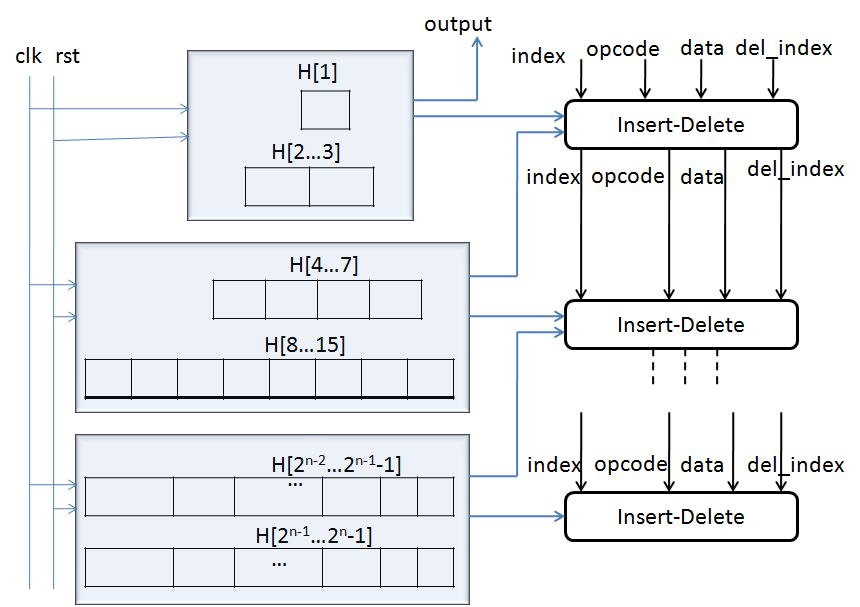
\includegraphics[width=7cm]{fig/d3.png}
      \caption{Sharing {\it Insert-Delete} hardware between two consecutive levels.}
    \label{d3}
\end{figure}

We have seen in Figure \ref{clock2} that for each level, there is an {\it idle} state.
For example, while level $L_2$ becomes idle at clock $3$ after performing {\it comp} at clock $2$.
This idle state occurs because $L_2$ is waiting on the result from level $L_3$ as the latter is performing {\it comp}.
Eventually, $L_2$ performs {\it write} at clock $4$ after the data becomes available by $L_3$.

While a level is in an idle state, no operation could be performed at that level at that time.
In general, for any given time $t$, the level $L_i$ cannot be completed if level $L_{i+1}$ cannot finish {\it comp} at $t+1$.
In this situation, we can share hardware between the levels $L_i$ and $L_{i+1}$, as shown in Figure \ref{d3}.

\subsubsection{Replacement Technique}
 There are four possible sequences of operations: {\it Insert-Only} ($I$), {\it Delete-Only} ($D$), {\it Insert-Delete} ($ID$) and {\it Delete-Insert} ($DI$).
The {\it Insert-Only} sequences ($I \ I \ \cdots I $) take single clock cycle to operate at each stage.
While our insert-delete logic minimizes holes created from $IDID \cdots DIDI \cdots$ sequences, we can optimize for scenarios where the insert or delete request immediately follows after the cycle where the other is encountered.
Here, we introduce a {\it replacement} operation that does not cause holes.
The algorithm of this operation is as follows:
 \begin{enumerate}
 \item Let $X$ be the root element and $Y$ be the element to insert from a request sequence $ID \cdots DI$.
 \item Delete $min(X, \ Y)$
 \item $H[1] \leftarrow min(X,\ Y)$
 \item Continue this replacement for each level by comparing $H[i]$ with $H[2i]$ and $H[2i+1]$, until the parent becomes less than its children, or it reaches to the leaf node.
 \end{enumerate}
The time complexity for these sequences is exactly the same as for {\it Insert-Only} where no holes are generated.
Our replacement operation is ignored if the second request occurs more than one cycle after the first.
Thus, this optimization can work in parallel with our hole minimization technique.
